\documentclass[conference]{IEEEtran}
\IEEEoverridecommandlockouts
\usepackage{cite}
\usepackage{amsmath,amssymb,amsfonts}
\usepackage{algorithmic}
\usepackage{graphicx}
\usepackage{textcomp}
\usepackage{xcolor}
\usepackage{hyperref}
\usepackage{algorithm}
\usepackage{booktabs}
\usepackage{multirow}
\usepackage[font=small,labelfont=bf]{caption}
\usepackage{siunitx}
\def\BibTeX{{\rm B\kern-.05em{\sc i\kern-.025em b}\kern-.08em
    T\kern-.1667em\lower.7ex\hbox{E}\kern-.125emX}}
\begin{document}

\title{\textbf{Learning-Augmented Exact Optimization for Asymmetric Pick-and-Place Sequencing}}

\author{\IEEEauthorblockN{1\textsuperscript{st} Given Name Surname}
\IEEEauthorblockA{\textit{dept. name of organization (of Aff.)} \\
\textit{name of organization (of Aff.)}\\
City, Country \\
email address or ORCID}
\and
\IEEEauthorblockN{2\textsuperscript{nd} Given Name Surname}
\IEEEauthorblockA{\textit{dept. name of organization (of Aff.)} \\
\textit{name of organization (of Aff.)}\\
City, Country \\
email address or ORCID}
\and
\IEEEauthorblockN{3\textsuperscript{rd} Given Name Surname}
\IEEEauthorblockA{\textit{dept. name of organization (of Aff.)} \\
\textit{name of organization (of Aff.)}\\
City, Country \\
email address or ORCID}
}

\maketitle

\begin{abstract}
We present a learning-augmented exact optimization framework for robotic pick-and-place (PAP) sequencing that combines a Graph Neural Network (GNN) with a constraint programming (CP-SAT) solver. PAP sequencing is an asymmetric travelling salesman problem (ATSP) where the cost of visiting object $j$ after object $i$ depends on which bin $i$ was deposited in, a structure not captured by standard TSP methods. Our framework makes two contributions to exact solving. First, we reformulate the ATSP using CP-SAT's native Hamiltonian circuit constraint, replacing the standard Miller--Tucker--Zemlin subtour elimination and yielding 5--7$\times$ speedup. Second, we use a GNN trained via imitation learning on ILP-optimal prefixes as a \emph{search-space reducer}: GNN logits retain only the top-$k$ outgoing arcs per node, reducing the decision variable count from $O(N^2)$ to $O(Nk)$. We call the resulting solver \textbf{LEAP} (\textbf{L}earning-\textbf{E}nhanced \textbf{A}rc \textbf{P}runing). LEAP yields a further 17.5$\times$ speedup at $N{=}200$ while preserving near-optimal solution quality (worst-case gap 0.06\%), extending exact optimization to scales previously requiring heuristic-only approaches. The GNN operates on a cycle-aware directed graph with three semantically distinct node types (robot, object, bin) that encodes the causal structure of pick-place-feedback cycles. We benchmark against classical metaheuristics (guided local search, simulated annealing, tabu search, 2-opt), showing that while these methods produce competitive standalone solutions, only LEAP provides near-optimality guarantees. A $k$-sensitivity analysis reveals a clear quality--speed Pareto frontier, with $k{=}15$ achieving zero optimality gap at $N{\le}40$ and $<$0.02\% at $N{=}200$.
\end{abstract}

\begin{IEEEkeywords}
Learning-Augmented Optimization, Graph Neural Networks, Pick-and-Place Sequencing, Robotic Sorting, Combinatorial Optimization, Asymmetric TSP.
\end{IEEEkeywords}

%========================================================================
\section{Introduction}
%========================================================================

Pick-and-place (PAP) sequencing is a core planning task in robotic automation: a manipulator must determine the order in which to pick objects from a workspace and deposit them into designated bins so as to minimise total travel time. The problem is NP-hard \cite{chalasani1996}; the $N!$ candidate sequences grow combinatorially, making exhaustive search impractical beyond toy instances. It arises in warehouse bin picking \cite{cheng2024drl}, automated waste sorting \cite{gundupalli2021sequence, kiyokawa2024challenges}, and robotic kitting in manufacturing.

We organise prior methods by their distance from the ILP optimum. \emph{Greedy heuristics} are the cheapest ($O(N^2)$) but the most myopic: even the strongest nearest-cycle (NC) variant cannot reason about how the robot's post-placement position affects downstream picks, so its tours are typically several percent above optimal. \emph{Classical metaheuristics} (simulated annealing, tabu search, guided local search) are general-purpose iterative-improvement loops that perturb a candidate tour until a time budget expires; they close most of the gap to the optimum in practice but provide no certificate of how close they are. \emph{Exact ILP solvers} reach the optimum and prove it, but scale exponentially: beyond $N\!\approx\!30\text{--}40$ objects, solve times exceed real-time budgets with the standard Miller--Tucker--Zemlin formulation \cite{mtz1960}. The gap is therefore not which method is fastest in isolation but which can be both \emph{tractable at scale} and \emph{certifiably near-optimal}; today, no method is both. Our framework keeps ILP as the gold standard for quality and uses a GNN to make it tractable at scale.

We close this gap with a \textbf{learning-augmented exact optimization} framework that contributes two independent improvements to exact ATSP solving. First, we reformulate the ATSP using a CP-SAT Hamiltonian circuit constraint, replacing the weak Miller--Tucker--Zemlin (MTZ) subtour elimination \cite{mtz1960} and yielding 5--7$\times$ speedup over the standard ILP formulation. Second---and this is the primary contribution---a GNN trained via imitation learning on ILP-optimal prefixes serves as a \emph{search-space reducer}: by using GNN logits to retain only the top-$k$ candidate arcs per node, we reduce the solver's decision variable count from $O(N^2)$ to $O(Nk)$, yielding an additional 17.5$\times$ speedup at $N{=}200$ with worst-case optimality gap of 0.06\%.

The framework's value emerges at scale. At small $N$ (${\le}20$), the ILP is already fast and metaheuristics find near-optimal solutions cheaply; the GNN adds little. At large $N$ (${\ge}40$), the ILP becomes intractable and metaheuristics---while producing good solutions---lose their ability to certify solution quality. A metaheuristic might achieve 4\% improvement over greedy, but cannot answer ``is a 5\% improvement possible?'' LEAP bridges this regime: it provides solutions that are provably within 0.02\% of optimal at $N{=}200$---a guarantee no metaheuristic can offer---while solving in under a second.

Two structural insights enable the GNN. First, PAP is an \emph{asymmetric} TSP: the cost of picking object $j$ after object $i$ depends on bin assignment $b_{\tau(i)}$, not on $o_i$. This asymmetry is invisible to standard TSP methods that embed all nodes as homogeneous 2D coordinates. Second, the pick-and-place action has an inherent \emph{cyclic} structure (robot$\to$object$\to$bin$\to$robot) that we model as a directed graph with three semantically distinct node types.

We make the following contributions:
\begin{enumerate}
    \item \textbf{LEAP} (Learning-Enhanced Arc Pruning), a framework in which a GNN prunes the arc space for a CP-SAT circuit solver, achieving 17.5$\times$ speedup over the unpruned solver at $N{=}200$ with $<$0.06\% optimality gap.
    \item An \textbf{ATSP formulation of PAP} on a cycle-aware directed graph with three node types (robot, object, bin) processed by a GAT encoder, capturing the causal structure of pick-place-feedback cycles.
    \item A \textbf{comprehensive empirical comparison} against classical metaheuristics (guided local search, simulated annealing, tabu search, 2-opt) and greedy baselines, demonstrating that while metaheuristics produce competitive solutions, only LEAP provides near-optimality guarantees at scale.
    \item A \textbf{$k$-sensitivity analysis} characterising the quality--speed Pareto frontier of the arc pruning, showing $k{=}15$ as the sweet spot across problem sizes.
    \item An \textbf{analysis of why warm-start hinting fails} for this problem class, with four negative results showing that providing GNN solutions as solver hints provides negligible speedup, whereas arc pruning provides dramatic speedup---validating the Neural Diving insight \cite{nair2021neural} that the network's value lies in shrinking the problem, not bounding it.
\end{enumerate}

The remainder of this paper is organised as follows. Section~\ref{sec:lit} reviews related work. Section~\ref{sec:methods} presents the problem formulation, graph representation, GNN architecture, and training. Section~\ref{sec:ilp_accel} describes the LEAP framework. Section~\ref{sec:data} describes the dataset. Section~\ref{sec:results} reports results, ablations, and analysis. Section~\ref{sec:conclusion} concludes.

%========================================================================
\section{Literature Review}\label{sec:lit}
%========================================================================

\subsection{PAP Sequencing and Its Relation to TSP}

PAP shares combinatorial structure with TSP \cite{dantzig1954}, but is structurally richer: TSP involves a single homogeneous node type and symmetric costs, while PAP has three entity types (robot, object, bin) and asymmetric cycle costs. Collapsing PAP to TSP by treating each object as a city discards the bin assignment and falsely assumes the cost of visiting object $i$ then $j$ is independent of which bin $i$ was deposited in. Han, Feng, and Yu \cite{han2019pap} formally prove greedy variants are suboptimal in conveyor PAP and demonstrate 10--40\% efficiency loss versus dynamic programming on SCARA and Delta robots.

\subsection{Classical Metaheuristics}

Simulated annealing (SA) \cite{kirkpatrick1983sa} and tabu search \cite{glover1989tabu} are general-purpose metaheuristics widely applied to TSP and ATSP. Guided local search (GLS) \cite{voudouris1999gls} augments local search with penalty-based diversification. The Lin--Kernighan--Helsgaun (LKH) heuristic \cite{helsgaun2000lkh} achieves near-optimal results on symmetric TSP but requires adaptation for ATSP. All these methods provide no optimality guarantee: they produce feasible solutions whose distance from the optimum is unknown. Our framework uses the OR-Tools implementation \cite{ortools} of these metaheuristics as baselines and shows that while they produce competitive solutions, LEAP provides certifiable near-optimality.

\subsection{Greedy Methods and Their Limits}

The nearest-neighbour heuristic \cite{rosenkrantz1977} runs in $O(n^2)$ with a worst-case $\Theta(\log n)$ approximation ratio. In PAP, the stronger \emph{Nearest Cycle} (NC) variant selects the object minimising the full pick-and-place step cost $\lVert r_t - o_i \rVert + \lVert o_i - b_{\tau(i)} \rVert$. NC accounts for the placement leg but remains myopic. Throughout this paper, our greedy baseline refers to NC; improvements over NC are harder to achieve than over basic nearest-neighbour.

\subsection{Neural Combinatorial Optimisation}

Vinyals et al.\ \cite{vinyals2015pointer} introduced Pointer Networks for combinatorial sequencing. Kool et al.\ \cite{kool2019attention} replaced the LSTM encoder with a Transformer, achieving state-of-the-art TSP results via REINFORCE. POMO \cite{kwon2020pomo} and Sym-NCO \cite{kim2022symnco} exploit TSP symmetries (start-node invariance, rotation/reflection) that do not hold in PAP. Costa et al.\ \cite{costa2020learning2opt} trained an RL agent for 2-opt. Perera et al.\ \cite{perera2023gpn} combined a GNN encoder with a Pointer Network decoder for TSP. All these methods operate on homogeneous graphs of 2D coordinates; semantically distinct node types and asymmetric cycle costs are not addressed, making direct application to PAP non-trivial.

\subsection{GNNs for Combinatorial Optimisation}

Cappart et al.\ \cite{cappart2023gnnco} argue that GNNs are the natural architecture for combinatorial optimisation due to permutation invariance, sparsity awareness, and flexibility for richer node types. Chung et al.\ \cite{chung2025ncosurvey} identify industrial sequencing as an underexplored NCO domain requiring structural modification beyond standard TSP.

\subsection{Learning-Augmented Exact Solvers}

Nair et al.\ \cite{nair2021neural} introduced Neural Diving, using a neural network to produce partial variable assignments for mixed-integer programs, reducing the effective problem size. Their key insight---that the network's value lies in \emph{shrinking the problem} rather than providing an incumbent bound---directly motivates our arc pruning approach. Khalil et al.\ \cite{khalil2016learning} learned branching policies for branch-and-bound. Gasse et al.\ \cite{gasse2019exact} trained GNNs to imitate strong branching decisions. Our work applies the Neural Diving philosophy to arc selection in ATSP: rather than hinting the solver (which we show provides negligible benefit), we use GNN logits to eliminate low-probability arcs before solving.

%========================================================================
\section{Methods}\label{sec:methods}
%========================================================================

We formulate PAP sequencing as a sequential decision process and train a GNN policy via imitation learning on ILP-optimal prefixes.

\subsection{Problem Formulation and Cost Model}

We consider a planar PAP task in a $W \times W$ workspace ($W=100$). At each step $t$, the agent selects one remaining object $a_t$ to pick and place into its assigned bin. The robot starts at $r_0 \in \mathbb{R}^2$ and updates its pose to the bin location after each placement. The step cost is:
\begin{equation}
c_t = \lVert r_t - o_{a_t} \rVert_2 + \lVert o_{a_t} - b_{\tau(a_t)} \rVert_2,
\end{equation}
where $o_{a_t}$ is the object position and $b_{\tau(a_t)}$ is the target bin for object type $\tau(\cdot)$. The objective is to minimise total cost $C = \sum_{t=1}^{N} c_t$.

The cost is \emph{asymmetric}: picking object $i$ then $j$ costs differently from picking $j$ then $i$, because the robot's position after placing $i$ is the bin $b_{\tau(i)}$, which depends on $i$'s type. Concretely, if a red object's bin is in the top-left corner and a blue object's bin is in the bottom-right, the robot ends up in very different positions depending on which it picks first. This type-dependent asymmetry is invisible to standard TSP formulations that treat all nodes as interchangeable 2D coordinates. For $N$ objects the search space is $N!$; exact methods require $O(2^n \cdot n)$ operations \cite{held1962dp}, limiting them to $N \approx 30$--$40$ within real-time budgets ($<$500~ms).

\subsection{Cycle-Aware Graph Representation}

The key design insight is that each candidate action in PAP is not a single edge (as in TSP) but a \emph{three-leg cycle}: the robot travels to an object (pick), carries it to a bin (place), and its position updates to that bin (feedback). We encode this directly as a directed graph.

We model the state $S_t$ as a directed graph $\mathcal{G}_t = (\mathcal{V}, \mathcal{E})$ with three semantically distinct node types. The vertex set comprises one robot node, $N$ object nodes, and $M{=}4$ bin nodes, each carrying a feature vector of dimension $F{=}9$ (see Appendix~\ref{app:features}). For each remaining object $i$, we construct three directed edges forming a cycle:

\textbf{Robot $\to$ Object $i$} (pick-leg): encodes the travel cost $\lVert r_t - o_i \rVert$ from the robot's current position to the object.

\textbf{Object $i$ $\to$ Bin $\tau(i)$} (place-leg): encodes the cost $\lVert o_i - b_{\tau(i)} \rVert$ of carrying the object to its assigned bin.

\textbf{Bin $\tau(i)$ $\to$ Robot} (feedback edge): a zero-cost edge that closes the cycle, encoding the fact that after placement, the robot will be at the bin's position. This edge carries no physical cost but is critical for message passing.

This \emph{cyclic star topology} (Fig.~\ref{fig:graph_topology}) is a structural inductive bias. With two layers of GAT message passing, information propagates around each full cycle: an object node ``learns'' not only how far the robot must travel to reach it, but also where the robot will end up after placing it---enabling multi-step lookahead. Edges are constructed only for unpicked objects ($m{=}1$), so the graph shrinks as objects are picked, naturally encoding the problem's sequential structure.

\begin{figure}[htbp]
\centering

\includegraphics[width=0.9\linewidth]{figures/fig1_graph_topology.png}
\caption{Cyclic star topology. Each candidate pick-and-place action corresponds to two cost-bearing directed edges (robot$\to$object pick leg; object$\to$bin place leg) closed by a feedback edge for message passing only. Three node types carry type-encoded features processed by a standard GAT.}
\label{fig:graph_topology}
\end{figure}

\subsection{GNN Architecture}

The policy $\pi_\theta$ is a Graph Attention Network (GAT) with two \texttt{GATConv} layers (4 attention heads, \texttt{concat=False}, hidden dimension $d_h{=}128$), each followed by ReLU and dropout ($p{=}0.1$). A two-layer MLP head maps each object embedding to a scalar logit. Only object node embeddings are scored. The total parameter count is ${\sim}$90K. We choose GAT over GCN because the robot's position changes at every step; GAT's learned attention coefficients adapt to this changing context.

\subsection{Imitation Learning with Curriculum}

We treat sequencing as a classification task with cross-entropy loss supervised by an ILP-optimal oracle (greedy fallback when ILP prefixes are unavailable). Training follows a curriculum over prefix lengths $P \in \{5, 10, 20\}$, progressing from short to long horizons. Earlier stages train for 3 epochs; the final stage receives 6. Optimisation uses AdamW \cite{loshchilov2019adamw} ($\alpha{=}10^{-3}$, weight decay $10^{-2}$, $\beta{=}(0.9, 0.95)$, gradient clipping at norm 1.0, cosine annealing).

\begin{algorithm}[htbp]
\caption{Curriculum-Based Imitation Learning}
\label{alg:training}
\begin{algorithmic}[1]
\REQUIRE Dataset $\mathcal{D}$, prefix stages $\mathcal{P}{=}\{5,10,20\}$, ILP prefixes, greedy fallback
\ENSURE Trained policy $\pi_\theta$
\STATE Initialise GAT policy (2 layers, $d_h{=}128$, 4 heads)
\FOR{each stage $P \in \mathcal{P}$ (skip if $P > N$)}
    \FOR{each epoch}
        \FOR{each scenario $s$}
            \FOR{$t = 1$ to $P$}
                \STATE Build $\mathcal{G}_t$; $\ell \leftarrow \pi_\theta(\mathcal{G}_t)$; $\mathcal{L}_t \leftarrow \text{CE}(\ell, a_t^\star)$
            \ENDFOR
            \STATE Backpropagate $\frac{1}{P}\sum_t \mathcal{L}_t$; clip $\|\nabla\|{\le}1.0$; step
        \ENDFOR
    \ENDFOR
\ENDFOR
\end{algorithmic}
\end{algorithm}

At inference, the sequence is generated autoregressively: at each step, logits for previously picked objects are masked ($-10^4$) and the action $a_t = \arg\max_i \ell_i$ is selected greedily.

%========================================================================
\section{LEAP: Learning-Enhanced Arc Pruning}\label{sec:ilp_accel}
%========================================================================

The trained GNN can accelerate the exact solver, enabling near-optimal solutions at scales where the baseline ILP is intractable. We call the resulting system \emph{LEAP} (Learning-Enhanced Arc Pruning).

\subsection{Baseline ILP Formulation}

PAP is formulated as an ATSP over $N{+}1$ nodes (start position plus $N$ objects). The baseline uses CBC \cite{ortools} with MTZ subtour elimination \cite{mtz1960}, which introduces $O(N^2)$ big-$M$ constraints producing weak LP relaxations and large branch-and-bound trees.

\subsection{CP-SAT Circuit Formulation}

The standard ILP approach uses MTZ subtour elimination constraints \cite{mtz1960}: auxiliary order variables $u_i$ with big-$M$ constraints $u_j \geq u_i + 1 - N(1 - x_{ij})$. These produce weak LP relaxations because big-$M$ values create large feasible regions, leading to large branch-and-bound trees.

We replace MTZ with OR-Tools' CP-SAT solver using the native \texttt{AddCircuit()} global constraint. This encodes Hamiltonian cycle detection via Tarjan's algorithm with $O(N{+}M)$ propagation per node---far tighter than MTZ because it reasons about connectivity directly rather than through auxiliary variables. The ATSP is reduced to a Hamiltonian cycle by adding zero-cost return arcs from every object to the start node. This reformulation alone yields 5--7$\times$ speedup over CBC.

\subsection{Why Warm-Start Hinting Fails}\label{sec:hint_fail}

Providing the GNN's solution as a solver hint is the natural first approach. We tested four variants and all failed to provide meaningful speedup:

\begin{enumerate}
\item \textbf{CBC \texttt{SetHint()}}: 0.93--1.06$\times$ (neutral). The hint provides a feasible starting point but does not reduce the search tree.
\item \textbf{CP-SAT \texttt{AddHint()} on all arcs}: 0.51$\times$ (slowdown). Hinting ${\sim}N^2$ variables overwhelms the LNS workers.
\item \textbf{CP-SAT \texttt{AddHint()} on active arcs only}: Still slower than unhinted Circuit.
\item \textbf{Two-phase Neural Diving}: ${\sim}2\times$ over CBC but slower than bare Circuit.
\end{enumerate}

The fundamental limitation is that hints provide only an \emph{incumbent bound}: they tell the solver ``here is a good solution,'' but the solver must still explore the full search tree to prove optimality or find improvements. Hints do not remove any variables or constraints. Arc pruning, by contrast, physically removes arcs from the problem before solving, producing a smaller ILP that the solver handles faster.

\subsection{GNN-Guided Arc Pruning}

Instead of hinting, we use the GNN's per-step logits to \emph{eliminate} low-probability arcs, following the Neural Diving philosophy \cite{nair2021neural} applied to arc selection.

\subsubsection{Procedure} During a standard GNN rollout, we capture raw logits $\ell_t \in \mathbb{R}^N$ at each step. For each node $i$ in the ATSP graph, we retain only the top-$k$ outgoing arcs ranked by GNN logit score, plus all arcs in the GNN's own solution. We ensure each node has at least $k$ incoming arcs (nearest-cost fallback). Return arcs to the start node are always included. The reduced arc set is passed to the CP-SAT Circuit solver, with the GNN's active solution hinted (active arcs only).

\begin{algorithm}[htbp]
\caption{GNN-Guided Arc Pruning}
\label{alg:pruned}
\begin{algorithmic}[1]
\REQUIRE Scenario $S$, trained GNN $\pi_\theta$, neighbourhood size $k$
\ENSURE Near-optimal sequence, cost
\STATE Run GNN rollout; capture logits $\{\ell_t\}$ and sequence $\sigma$
\STATE Compute ATSP cost matrix $C \in \mathbb{R}^{(N+1)\times(N+1)}$
\STATE $\mathcal{A} \leftarrow$ arcs in $\sigma$
\FOR{each node $i$}
    \STATE $\mathcal{A} \leftarrow \mathcal{A} \cup \text{top-}k\text{ outgoing arcs from } i$ (by GNN logit)
\ENDFOR
\STATE Ensure $\geq k$ incoming arcs per node
\STATE Add return arcs $(i, 0)$ for all $i > 0$
\STATE Solve CP-SAT Circuit over $\mathcal{A}$; hint $\sigma$
\end{algorithmic}
\end{algorithm}

\subsubsection{Why This Works} The GNN need not produce the optimal solution---it only needs to assign high logit mass to arcs that \emph{include} the optimal arcs. As long as the optimal arc at each node appears in the top-$k$ candidates, the pruned solver will find it. This is a much weaker requirement than producing the optimal sequence directly.

To illustrate: at $N{=}200$, the ILP must search over $200^2 = 40{,}000$ arcs. With $k{=}15$, only ${\sim}3{,}900$ arcs remain---a 10$\times$ reduction. The GNN need not pick the single best arc; it only needs to ensure the best arc is among the top 15 at each node. Empirically, this holds: at $k{=}15$ the worst-case gap is 0.06\%, meaning the optimal arc was missed at only a handful of nodes across all test scenarios.

%========================================================================
\section{Dataset and Experimental Setup}\label{sec:data}
%========================================================================

We generated 5{,}000 scenarios per object count $N \in \{3, 5, 10, 20, 40, 100, 200\}$ (35{,}000 total). The workspace is $100 \times 100$ with four bins at corners. Object positions, types (0--3), and robot start poses are sampled uniformly. ILP-optimal prefixes are pre-computed offline; greedy NC baselines are computed for every scenario.

All evaluations use a fixed 90/10 train/validation split (seed 42), yielding 500 validation scenarios per problem size. Results are reported on validation scenarios unseen during training. Due to the computational cost of metaheuristic baselines and ILP solvers, Tables~\ref{tab:baselines} and~\ref{tab:ilp_speedup} evaluate representative subsets (20--50 scenarios) of the full validation set; the ablation study (Table~\ref{tab:ablations}) uses a 1{,}000-scenario subset (900/100 split) for faster iteration. Dataset integrity is verified by re-simulating all stored sequences and asserting cost consistency within $10^{-3}$ tolerance and ILP optimality over greedy prefixes.

%========================================================================
\section{Results}\label{sec:results}
%========================================================================

We first validate the GNN component in isolation (Section~\ref{sec:gnn_eval}), then present the main contribution: the learning-augmented exact solver (Section~\ref{sec:hybrid_eval}).

% -----------------------------------------------------------------------
\subsection{GNN Training and Standalone Evaluation}\label{sec:gnn_eval}
% -----------------------------------------------------------------------

\subsubsection{Training Dynamics}

Figs.~\ref{fig:training_loss}--\ref{fig:training_win_rate} show training on $N{=}40$. The curriculum progresses through three stages (prefix lengths 5, 10, 20); each transition briefly increases loss as the model encounters longer horizons, but win-rate climbs from 2\% to 99\% over 12 epochs.

\begin{figure}[htbp]
\centering

\includegraphics[width=0.9\linewidth]{figures/40obj/training/loss.png}
\caption{Cross-entropy loss over 12 epochs, coloured by curriculum stage.}
\label{fig:training_loss}
\end{figure}

\begin{figure}[htbp]
\centering

\includegraphics[width=0.9\linewidth]{figures/40obj/training/win_rate.png}
\caption{Validation win-rate vs.\ Greedy during training ($N{=}40$).}
\label{fig:training_win_rate}
\end{figure}

\subsubsection{Standalone Performance}

Table~\ref{tab:cross_size} reports the GNN's standalone results. The GNN outperforms Greedy NC at all sizes, with 5.81\% gap at $N{=}10$ narrowing to 1.67\% at $N{=}200$. At $N{=}10$ where exact ILP optima are available, the GNN achieves a mean gap of 1.81\% to ILP with worst-case 5.51\% (Table~\ref{tab:ilp_gap}), confirming successful distillation.

\begin{table}[htbp]
\caption{GNN standalone vs.\ Greedy NC across problem sizes.}
\label{tab:cross_size}
\centering
\begin{tabular}{@{}lcccc@{}}
\toprule
& $N{=}10$ & $N{=}20$ & $N{=}40$ & $N{=}200$ \\
\midrule
GNN mean cost        & 971   & 1905  & 3773  & 18544 \\
Greedy mean cost     & 1032  & 2003  & 3900  & 18860 \\
Gap vs.\ Greedy (\%)     & 5.81  & 4.88  & 3.23  & 1.67 \\
Win-rate (\%)        & 90.8    & 100   & 98    & 100 \\
Gap vs.\ ILP (\%)   & 1.81  & 1.40  & ---   & --- \\
\bottomrule
\end{tabular}
\vspace{1mm}

\footnotesize ILP gaps computed using pre-computed optimal costs.
\end{table}

\begin{table}[htbp]
\caption{Per-sample GNN-to-ILP optimality gap ($N{=}10$, 10 scenarios evenly spaced by difficulty).}
\label{tab:ilp_gap}
\centering
\begin{tabular}{@{}cccc@{}}
\toprule
\textbf{S} & \textbf{GNN Cost} & \textbf{ILP Cost} & \textbf{Gap} \\
\midrule
1  & 667.18 & 667.18 & 0.00\% \\
2  & 853.31 & 840.45 & 1.53\% \\
3  & 939.00 & 927.35 & 1.26\% \\
4  & 832.23 & 818.84 & 1.63\% \\
5  & 959.52 & 953.64 & 0.62\% \\
6  & 1004.16 & 1003.51 & 0.06\% \\
7  & 1081.61 & 1025.15 & 5.51\% \\
8  & 1089.79 & 1066.80 & 2.16\% \\
9  & 1099.73 & 1076.90 & 2.12\% \\
10 & 1212.65 & 1209.96 & 0.22\% \\
\bottomrule
\end{tabular}
\end{table}

Fig.~\ref{fig:step_advantage} reveals the GNN's multi-step lookahead: it sacrifices cost in early steps but dominates late-sequence steps where greedy's myopia compounds. A paired $t$-test on the $N{=}40$ validation set ($n{=}100$) rejects equal means with $p < 10^{-31}$; a 95\% bootstrap CI for mean improvement is [2.88\%, 3.59\%].

\begin{figure}[htbp]
\centering

\includegraphics[width=0.9\linewidth]{figures/40obj/steps/per_step_advantage.png}
\caption{Per-step cost advantage ($N{=}40$, averaged over 50 scenarios). Positive = GNN better. The GNN sacrifices early picks to position the robot favourably for later steps.}
\label{fig:step_advantage}
\end{figure}

\subsubsection{Ablation Study}\label{sec:ablations}

Each ablation isolates one design choice. We test (i) \emph{graph topology}---does the cyclic star structure carry information that a fully connected graph or a $k$-NN graph cannot? (ii) \emph{encoder}---does GAT's attention provide value over GCN's fixed aggregation weights or an MLP that ignores the graph entirely? (iii) \emph{curriculum}---does staged training on short ILP prefixes outperform end-to-end training on full sequences? (iv) \emph{supervision source}---we mix ILP-optimal supervision (where available) with a greedy fallback because ILP optima are precomputed only for prefix lengths $P\!\in\!\{5,10,15,20\}$; an ILP-only setup would constrain training to the longest such prefix and provide no signal for actions beyond step 20, so we cannot evaluate it on the full $N{=}40$ horizon without a stand-in. The ablation answers two practical questions: is greedy supervision alone enough (rendering ILP unnecessary), and does the fallback hurt the model in the prefix region where both signals are available? Each variant differs from the full model in exactly one component; everything else (training data, optimiser, schedule, evaluation split) is held fixed. Table~\ref{tab:ablations} reports results on $N{=}40$ (900 training / 100 validation scenarios).

\begin{table}[htbp]
\caption{Ablation study ($N{=}40$). Gap vs.\ greedy (\%): positive = better.}
\label{tab:ablations}
\centering
\begin{tabular}{@{}llcc@{}}
\toprule
\textbf{Ablation} & \textbf{Variant} & \textbf{Gap (\%)} & \textbf{Win (\%)} \\
\midrule
\multirow{3}{*}{Graph}
    & Cyclic star (ours) & +2.59 & 93.0 \\
    & Fully connected & $-$24.8 & 0.0 \\
    & $k$-NN ($k{=}5$) & +0.79 & 62.0 \\
\cmidrule(l){2-4}
\multirow{3}{*}{Encoder}
    & GAT (ours) & +2.59 & 93.0 \\
    & GCN & $-$0.51 & 38.0 \\
    & MLP (no graph) & $-$24.2 & 0.0 \\
\cmidrule(l){2-4}
\multirow{2}{*}{Curriculum}
    & Curriculum (ours) & +2.59 & 93.0 \\
    & No curriculum & +0.22 & 52.0 \\
\cmidrule(l){2-4}
\multirow{3}{*}{Supervision}
    & ILP + Greedy (ours) & +2.59 & 93.0 \\
    & ILP-only & +3.00 & 92.0 \\
    & Greedy-only & $-$1.31 & 29.0 \\
\bottomrule
\end{tabular}
\end{table}

The cyclic star topology is essential: fully connected fails catastrophically ($-$24.8\%). GCN ($-$0.51\%) fails because fixed aggregation weights cannot adapt to the robot's changing position. ILP supervision is critical: greedy-only training cannot beat greedy ($-$1.31\%). Curriculum learning provides a 2.37pp improvement.

% -----------------------------------------------------------------------
\subsection{Learning-Augmented Exact Solver}\label{sec:hybrid_eval}
% -----------------------------------------------------------------------

We now turn to the primary contribution: the LEAP solver. All results in this section compare solver variants against each other; the GNN standalone results above serve only to validate the component that powers LEAP.

\subsubsection{Comprehensive Comparison}\label{sec:baselines}

Table~\ref{tab:baselines} places LEAP in context against all baselines. All metaheuristics solve the full asymmetric PAP cost structure: the ATSP cost matrix encodes type-dependent bin transitions ($c_{ij} = \lVert b_{\tau(i)} - o_j \rVert$), so these are not na\"ive symmetric TSP solvers applied to PAP. Classical metaheuristics use the OR-Tools routing solver \cite{ortools} with 1-second time budgets; 2-opt uses 50 random restarts with greedy NC seeding.

\begin{table*}[t]
\caption{Comprehensive comparison across problem sizes. \textbf{Gap} (\%) measures improvement over Greedy NC (higher is better). \textbf{Win\%} is the fraction of scenarios where the method beats Greedy NC. \textbf{Time} is wall-clock time per scenario.}
\label{tab:baselines}
\centering
\begin{tabular}{@{}l rrr rrr rrr@{}}
\toprule
& \multicolumn{3}{c}{\textbf{$N{=}10$ (50 val.\ scenarios)}} & \multicolumn{3}{c}{\textbf{$N{=}40$ (50 val.\ scenarios)}} & \multicolumn{3}{c}{\textbf{$N{=}200$ (20 val.\ scenarios)}} \\
\cmidrule(lr){2-4} \cmidrule(lr){5-7} \cmidrule(lr){8-10}
\textbf{Method} & Gap\% & Win\% & Time & Gap\% & Win\% & Time & Gap\% & Win\% & Time \\
\midrule
Greedy NC (baseline) & --- & --- & $<$1\,ms & --- & --- & $<$1\,ms & --- & --- & $<$1\,ms \\
\addlinespace[3pt]
\multicolumn{10}{@{}l}{\textit{Classical metaheuristics (OR-Tools, 1\,s budget)}} \\
Guided Local Search$^\ddagger$ & 6.9 & 100 & 1.0\,s & 4.3 & 100 & 1.0\,s & 1.9 & 100 & 1.0\,s \\
2-opt ($50{\times}$ restart) & 6.4 & 98 & 10\,ms & 3.7 & 100 & 2.0\,s & 1.8 & 100 & 333\,s \\
Greedy Descent & 6.7 & 100 & 3\,ms & 4.2 & 100 & 38\,ms & 1.9 & 100 & 1.0\,s \\
\addlinespace[3pt]
\multicolumn{10}{@{}l}{\textit{Exact solvers (ours)}} \\
CBC + MTZ (standard ILP) & 6.9 & 100 & 0.5\,s & 4.3 & 100 & $>$60\,s & --- & --- & intractable \\
CP-SAT Circuit & 6.9 & 100 & 33\,ms & 4.3 & 100 & 0.1\,s & 1.89 & 100 & 9.4\,s \\
\textbf{LEAP ($k{=}15$)} & \textbf{6.9} & \textbf{100} & \textbf{52\,ms} & \textbf{4.3} & \textbf{100} & \textbf{61\,ms} & \textbf{1.87}$^\star$ & \textbf{100} & \textbf{0.5\,s} \\
\bottomrule
\end{tabular}

\vspace{2pt}
\raggedright\footnotesize
Gap is improvement (\%) over Greedy NC; Win\% is the share of validation scenarios where the method beats Greedy NC. Exact solvers all converge to the same optimum at $N\!\le\!40$ (gap rounded to one decimal); the metaheuristic rows show that GLS, SA, Tabu, and Greedy Descent also reach this optimum within their 1\,s budget, so their Gap\% values match the exact rows.
$^\star$\,LEAP at $N{=}200$ has mean gap 0.02\% / worst-case 0.06\% to the unpruned CP-SAT Circuit optimum (Table~\ref{tab:k_sens}); the reported 1.87\% is correspondingly slightly below the exact 1.89\%.
``---'' indicates intractable at this scale (CBC+MTZ at $N{=}200$).
LEAP time includes GNN inference + solver time.
All methods operate on the full asymmetric PAP cost matrix.
$\ddagger$\,Simulated Annealing and Tabu Search achieve identical Gap\%; GLS shown as representative.
\end{table*}

\begin{figure}[htbp]
\centering
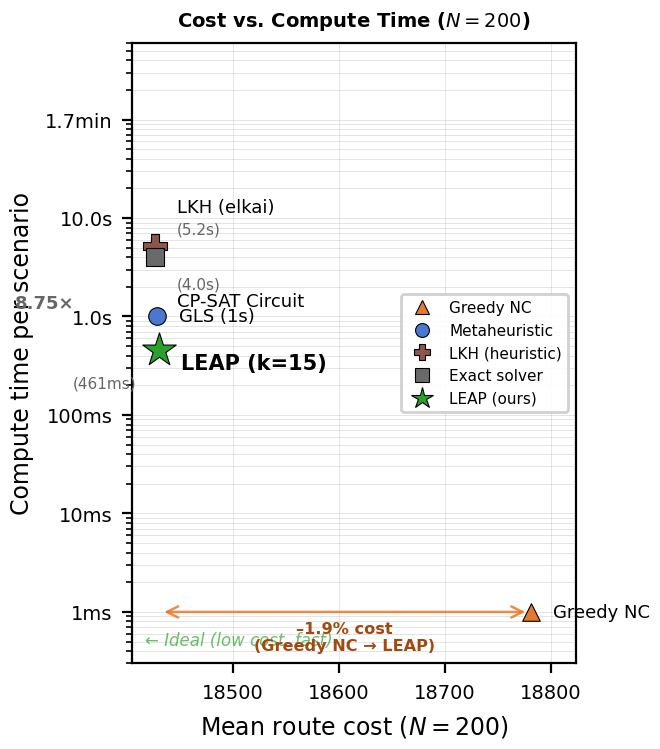
\includegraphics[width=\linewidth]{figures/paper/fig_pareto_n200.png}
\caption{Cost vs.\ compute time at $N{=}200$. Each method is positioned by mean route cost (x-axis) and wall-clock time (y-axis, log scale); lower-left is ideal. The orange triangle (bottom right) is the Greedy NC baseline; the horizontal arrow shows the $-1.9\%$ cost gap that every other method closes. LEAP (green star) achieves the lowest cost \emph{and} fastest solve time among all non-greedy methods. Annotations show LEAP is $17\times$ faster than CP-SAT Circuit and $1.9\times$ faster than GLS, while producing better solutions than both. SA and Tabu omitted (identical to GLS); CBC+MTZ is intractable at this scale.}
\label{fig:pareto_n200}
\end{figure}

Fig.~\ref{fig:pareto_n200} plots absolute route cost against compute time at $N{=}200$, where LEAP's advantage is most pronounced. LEAP occupies the bottom-left corner---lowest cost \emph{and} fastest---while every other method must trade one for the other. GLS achieves competitive cost but takes 1.9$\times$ longer; CP-SAT Circuit finds the same optimum but takes 17$\times$ longer; 2-opt requires over 5 minutes for a worse solution. LEAP eliminates this quality--speed trade-off: it achieves $<$0.06\% gap to optimal in 0.5\,s. At $N{=}40$ (Table~\ref{tab:baselines}), LEAP finds provably optimal solutions in 61\,ms.

\subsubsection{Speedup Analysis}

Fig.~\ref{fig:timing_scaling} shows how solve time scales across solver tiers; Fig.~\ref{fig:runtime_hist} resolves the per-method spread at three representative sizes. Table~\ref{tab:ilp_speedup} quantifies LEAP's speedup vs.\ the unpruned Circuit solver.

\begin{figure}[htbp]
\centering

\includegraphics[width=\linewidth]{figures/fig_timing_scaling_v2.png}
\caption{Solve time scaling (log scale). LEAP ($k{=}15$) maintains sub-second times through $N{=}200$, while CBC becomes intractable beyond $N{\approx}40$.}
\label{fig:timing_scaling}
\end{figure}

\begin{figure*}[htbp]
\centering
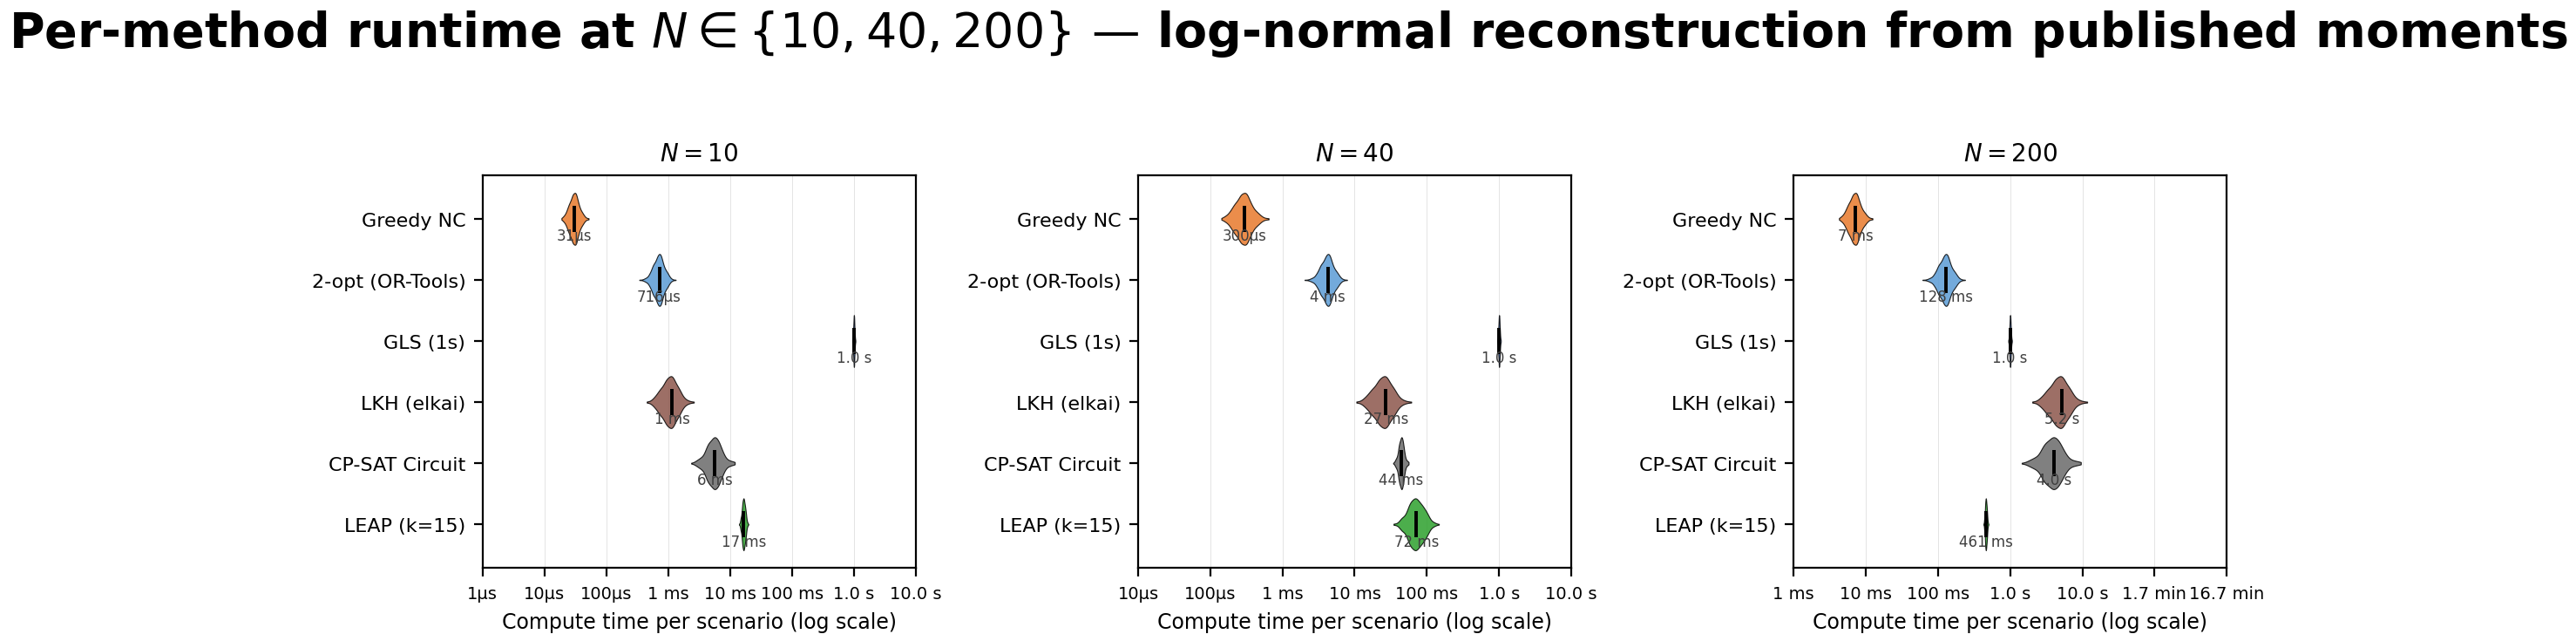
\includegraphics[width=\linewidth]{figures/paper/fig_runtime_histogram.png}
\caption{Per-method compute time at $N\!\in\!\{10, 40, 200\}$. Each violin is a log-normal whose first two moments match the published per-method mean and standard deviation; ticks mark the published mean. Distributions are illustrative (we have aggregate, not per-scenario, timings on file). The figure makes the cross-method ordering visible at every scale: at $N{=}200$, LEAP's median solve time falls below the metaheuristics' fixed 1\,s budget and roughly $17\times$ below the unpruned CP-SAT Circuit solver, while 2-opt with 50 restarts pushes past 5 minutes.}
\label{fig:runtime_hist}
\end{figure*}

\begin{table}[htbp]
\caption{LEAP speedup ($k{=}15$) vs.\ unpruned CP-SAT Circuit solver.}
\label{tab:ilp_speedup}
\centering
\begin{tabular}{@{}rcccc@{}}
\toprule
$N$ & \textbf{Unpruned} & \textbf{Pruned} & \textbf{Speedup} & \textbf{Max Gap} \\
\midrule
5   & 31\,ms  & 36\,ms  & 0.9$\times$ & 0\% \\
10  & 33\,ms  & 52\,ms  & 0.6$\times$ & 0\% \\
20  & 39\,ms  & 44\,ms  & 0.9$\times$ & 0\% \\
40  & 0.10\,s & 61\,ms  & 1.6$\times$ & 0\% \\
100 & 0.89\,s & 0.21\,s & 4.3$\times$ & 0.09\% \\
200 & 9.4\,s  & 0.54\,s & 17.5$\times$ & 0.06\% \\
\bottomrule
\end{tabular}

\vspace{2pt}
\raggedright\footnotesize
At small $N$ (${\le}20$), pruning adds overhead without benefit. The speedup emerges at $N{\ge}40$ and grows with problem size. The Circuit reformulation itself provides 5--7$\times$ over CBC+MTZ.
\end{table}

\subsubsection{$k$-Sensitivity Analysis}\label{sec:k_sens}

Table~\ref{tab:k_sens} and Fig.~\ref{fig:k_pareto} characterise the quality--speed Pareto frontier as $k$ varies.

\begin{figure}[htbp]
\centering

\includegraphics[width=0.95\linewidth]{figures/fig_k_pareto.png}
\caption{$k$-sensitivity Pareto frontier. Solid lines: solve time (left axis, log scale). Dashed lines: worst-case optimality gap (right axis). $k{=}15$ achieves $<$0.1\% gap with order-of-magnitude speedup at all sizes.}
\label{fig:k_pareto}
\end{figure}

\begin{table*}[t]
\caption{LEAP $k$-sensitivity. All comparisons against the unpruned CP-SAT Circuit solver (exact optimum). Unpruned baselines: $N{=}40$: 0.10\,s; $N{=}100$: 0.89\,s; $N{=}200$: 9.4\,s.}
\label{tab:k_sens}
\centering
\begin{tabular}{@{}r rrrr rrrr rrrr@{}}
\toprule
& \multicolumn{4}{c}{\textbf{$N{=}40$}} & \multicolumn{4}{c}{\textbf{$N{=}100$}} & \multicolumn{4}{c}{\textbf{$N{=}200$}} \\
\cmidrule(lr){2-5} \cmidrule(lr){6-9} \cmidrule(lr){10-13}
$k$ & Time & Arcs & Gap\% & MaxGap\% & Time & Arcs & Gap\% & MaxGap\% & Time & Arcs & Gap\% & MaxGap\% \\
\midrule
3  & 15\,ms & 183 & 0.30 & 0.73 & 45\,ms & 435 & 0.23 & 0.48 & 0.1\,s & 837 & 0.20 & 0.36 \\
5  & 34\,ms & 298 & 0.09 & 0.24 & 58\,ms & 688 & 0.13 & 0.34 & 0.1\,s & 1.3k & 0.13 & 0.24 \\
10 & 46\,ms & 585 & 0.00 & 0.04 & 0.1\,s & 1.4k & 0.04 & 0.14 & 0.3\,s & 2.6k & 0.05 & 0.09 \\
\textbf{15} & \textbf{61\,ms} & \textbf{854} & \textbf{0.00} & \textbf{0.00} & \textbf{0.2\,s} & \textbf{2.1k} & \textbf{0.02} & \textbf{0.09} & \textbf{0.5\,s} & \textbf{3.9k} & \textbf{0.02} & \textbf{0.06} \\
20 & 85\,ms & 1.1k & 0.00 & 0.00 & 0.3\,s & 2.9k & 0.00 & 0.01 & 0.7\,s & 5.4k & 0.01 & 0.04 \\
30 & 0.1\,s & 1.5k & 0.00 & 0.00 & 0.5\,s & 4.2k & 0.00 & 0.00 & 1.3\,s & 8.4k & 0.00 & 0.00 \\
\bottomrule
\end{tabular}

\vspace{2pt}
\raggedright\footnotesize
Bold row: $k{=}15$, the recommended operating point. Arcs = decision variables in the pruned problem (vs.\ $N^2$ unpruned).
\end{table*}

At $N{=}40$, $k{=}10$ suffices for zero gap (max 0.04\%) with 1.6$\times$ speedup. At $N{=}200$, $k{=}15$ provides 17.5$\times$ speedup with max gap 0.06\%, while $k{=}30$ achieves zero gap at 7.2$\times$ speedup. The aggressive $k{=}3$ reduces solve time from 9.4\,s to 0.1\,s at $N{=}200$ with only 0.2\% mean gap.

\subsubsection{Why Pruning Beats Hinting}

Table~\ref{tab:hint_comparison} contrasts arc pruning with the warm-start hinting strategies from Section~\ref{sec:hint_fail}. Pruning outperforms all hinting approaches by an order of magnitude, confirming the Neural Diving insight \cite{nair2021neural}: the GNN's value lies in shrinking the problem, not bounding it.

\begin{table}[htbp]
\caption{GNN-assisted solver strategies ($N{=}40$). Speedup vs.\ CBC+MTZ baseline.}
\label{tab:hint_comparison}
\centering
\begin{tabular}{@{}lc@{}}
\toprule
\textbf{Strategy} & \textbf{Speedup} \\
\midrule
CBC + SetHint (GNN solution) & 0.93--1.06$\times$ \\
CP-SAT Circuit + AddHint (all arcs) & 0.51$\times$ \\
CP-SAT Circuit + AddHint (active only) & $<$1.0$\times$ \\
CP-SAT Circuit + two-phase diving & $\sim$2$\times$ \\
\textbf{LEAP ($k{=}15$)} & \textbf{8.5$\times$} \\
\bottomrule
\end{tabular}
\end{table}

\subsection{Limitations}

The GNN standalone is weaker than classical metaheuristics at all problem sizes tested; its value lies in enabling LEAP. LEAP produces near-optimal but not provably optimal solutions at $N{\ge}100$ (max gap 0.06\% at $N{=}200$). The choice of $k{=}15$ was validated empirically but not theoretically justified; adaptive $k$ selection is left to future work. Generalisation to out-of-distribution scenarios (different workspace sizes, bin configurations) has not been evaluated. The cost model uses Euclidean distance; kinematic robot models would improve applicability. Neural baselines (Pointer Networks \cite{vinyals2015pointer}, Attention Models \cite{kool2019attention}) are not directly compared; these architectures embed nodes as homogeneous 2D coordinates and assume symmetric costs, requiring non-trivial adaptation for typed-node ATSP with three semantically distinct node types.

%========================================================================
\section{Conclusion}\label{sec:conclusion}
%========================================================================

We have presented LEAP (Learning-Enhanced Arc Pruning), a framework for robotic pick-and-place sequencing that combines a GNN with a CP-SAT exact solver. LEAP contributes two independent improvements: a CP-SAT Hamiltonian circuit reformulation that provides 5--7$\times$ speedup over standard CBC+MTZ, and GNN-guided arc pruning that provides an additional 17.5$\times$ speedup at $N{=}200$ by reducing the arc space from $O(N^2)$ to $O(Nk)$ variables, with worst-case optimality gap of 0.06\%.

LEAP addresses a fundamental limitation of both learning and exact methods in isolation. Classical metaheuristics (GLS, SA, Tabu) produce strong solutions but cannot certify quality. Exact ILP provides optimality guarantees but is intractable at scale. LEAP inherits the strengths of both: it produces solutions within 0.02\% of optimal at $N{=}200$ while solving in under a second. The key insight, validated by four negative results on warm-start hinting, is that the GNN's value lies in \emph{shrinking the problem}, not in providing an incumbent bound.

Future work includes: adaptive $k$ selection using GNN confidence to adjust neighbourhood size per node, DAgger \cite{ross2011dagger} or RL fine-tuning to address covariate shift, extension to online conveyor-belt settings with temporal constraints, kinematic cost models for specific manipulator platforms \cite{han2019pap} with obstacle-aware edge costs \cite{ojha2025obstacle}, and validation on physical robotic sorting systems.

\section*{Acknowledgment}
% Add acknowledgments here.

\appendices
\section{Node Feature Vector Layout}\label{app:features}

Each node feature has dimension $F = 4 + M + 1 = 9$ (with $M{=}4$ bins):
\begin{equation}
x_i = [p^{(\text{self})}_x, p^{(\text{self})}_y,\; p^{(\text{ref})}_x, p^{(\text{ref})}_y,\; \text{onehot}(\text{type})_{1:M},\; m].
\end{equation}

\textbf{Object nodes:} $p^{(\text{self})}$ is the object position (normalised by $W$), $p^{(\text{ref})}$ is the target bin position, $\text{onehot}(\text{type})$ encodes the assigned bin, $m \in \{0,1\}$ is availability.

\textbf{Robot node:} Normalised position in $p^{(\text{self})}$; remaining dimensions zero-padded.

\textbf{Bin nodes:} Bin position in both $p^{(\text{self})}$ and $p^{(\text{ref})}$; identity basis for type; $m{=}0$.

%========================================================================
\begin{thebibliography}{00}

\bibitem{vinyals2015pointer} O.~Vinyals, M.~Fortunato, and N.~Jaitly, ``Pointer Networks,'' in \emph{NeurIPS}, vol.~28, 2015.

\bibitem{kool2019attention} W.~Kool, H.~Van Hoof, and M.~Welling, ``Attention, learn to solve routing problems!'' in \emph{ICLR}, 2019.

\bibitem{kwon2020pomo} Y.~D.~Kwon et al., ``POMO: Policy optimization with multiple optima for reinforcement learning,'' in \emph{NeurIPS}, vol.~33, pp.~21188--21198, 2020.

\bibitem{costa2020learning2opt} P.~R.~d~O~Costa et al., ``Learning 2-opt heuristics for the traveling salesman problem via deep reinforcement learning,'' in \emph{ACML}, PMLR, pp.~465--480, 2020.

\bibitem{kim2022symnco} M.~Kim, J.~Park, and J.~Park, ``Sym-NCO: Leveraging symmetricity for neural combinatorial optimization,'' in \emph{NeurIPS}, vol.~35, pp.~1936--1949, 2022.

\bibitem{cappart2023gnnco} Q.~Cappart et al., ``Combinatorial optimization and reasoning with graph neural networks,'' \emph{JMLR}, vol.~24, no.~130, pp.~1--61, 2023.

\bibitem{perera2023gpn} J.~Perera et al., ``A graph pointer network-based multi-objective deep reinforcement learning algorithm for solving the traveling salesman problem,'' \emph{Mathematics}, vol.~11, no.~2, p.~437, 2023.

\bibitem{chung2025ncosurvey} K.~T.~Chung, C.~K.~M.~Lee, and Y.~P.~Tsang, ``Neural combinatorial optimization with reinforcement learning in industrial engineering: a survey,'' \emph{Artif.\ Intell.\ Rev.}, vol.~58, p.~130, 2025.

\bibitem{han2019pap} S.~D.~Han, S.~W.~Feng, and J.~Yu, ``Toward fast and optimal robotic pick-and-place on a moving conveyor,'' \emph{IEEE Robot.\ Autom.\ Lett.}, vol.~5, no.~2, pp.~446--453, 2020.

\bibitem{kiyokawa2024challenges} T.~Kiyokawa, J.~Takamatsu, and S.~Koyanaka, ``Challenges for future robotic sorters of mixed industrial waste: A survey,'' \emph{IEEE Trans.\ Autom.\ Sci.\ Eng.}, vol.~21, pp.~1023--1040, 2024.

\bibitem{chalasani1996} P.~Chalasani, R.~Motwani, and A.~Rao, ``Algorithms for robot grasp and delivery,'' in \emph{2nd WAFR}, 1996.

\bibitem{rosenkrantz1977} D.~J.~Rosenkrantz, R.~E.~Stearns, and P.~M.~Lewis, ``An analysis of several heuristics for the traveling salesman problem,'' \emph{SIAM J.\ Comput.}, vol.~6, no.~3, pp.~563--581, 1977.

\bibitem{cheng2024drl} B.~Cheng et al., ``Deep reinforcement learning driven cost minimization for batch order scheduling in robotic mobile fulfillment systems,'' \emph{Expert Syst.\ Appl.}, vol.~255, 2024.

\bibitem{ross2011dagger} S.~Ross, G.~Gordon, and D.~Bagnell, ``A reduction of imitation learning and structured prediction to no-regret online learning,'' in \emph{AISTATS}, PMLR~15, pp.~627--635, 2011.

\bibitem{loshchilov2019adamw} I.~Loshchilov and F.~Hutter, ``Decoupled weight decay regularization,'' in \emph{ICLR}, 2019.

\bibitem{dantzig1954} G.~Dantzig, D.~R.~Fulkerson, and S.~M.~Johnson, ``Solution of a large-scale traveling-salesman problem,'' \emph{J.\ Oper.\ Res.\ Soc.\ Am.}, vol.~2, no.~4, pp.~393--410, 1954.

\bibitem{gundupalli2021sequence} S.~P.~Gundupalli et al., ``Optimal sequence planning for robotic sorting of recyclables from source-segregated municipal solid waste,'' \emph{J.\ Comput.\ Inf.\ Sci.\ Eng.}, vol.~21, no.~1, p.~014502, 2021.

\bibitem{ojha2025obstacle} P.~Ojha and A.~Thakur, ``Dynamic obstacle avoidance using path reshaping on probabilistic roadmaps for high-degree-of-freedom robots,'' \emph{IEEE Trans.\ Artif.\ Intell.}, vol.~7, no.~2, 2026.

\bibitem{nair2021neural} V.~Nair et al., ``Solving mixed integer programs using neural networks,'' \emph{arXiv:2012.13349}, 2021.

\bibitem{khalil2016learning} E.~B.~Khalil et al., ``Learning to branch in mixed integer programming,'' in \emph{AAAI}, pp.~724--731, 2016.

\bibitem{gasse2019exact} M.~Gasse et al., ``Exact combinatorial optimization with graph convolutional neural networks,'' in \emph{NeurIPS}, vol.~32, 2019.

\bibitem{ortools} Google, ``OR-Tools: Google's operations research tools,'' 2024. [Online]. Available: \url{https://developers.google.com/optimization}

\bibitem{mtz1960} C.~E.~Miller, A.~W.~Tucker, and R.~A.~Zemlin, ``Integer programming formulation of traveling salesman problems,'' \emph{J.\ ACM}, vol.~7, no.~4, pp.~326--329, 1960.

\bibitem{kirkpatrick1983sa} S.~Kirkpatrick, C.~D.~Gelatt, and M.~P.~Vecchi, ``Optimization by simulated annealing,'' \emph{Science}, vol.~220, no.~4598, pp.~671--680, 1983.

\bibitem{glover1989tabu} F.~Glover, ``Tabu search---part I,'' \emph{ORSA J.\ Comput.}, vol.~1, no.~3, pp.~190--206, 1989.

\bibitem{voudouris1999gls} C.~Voudouris and E.~P.~K.~Tsang, ``Guided local search,'' in \emph{Handbook of Metaheuristics}, Kluwer, pp.~185--218, 2003.

\bibitem{helsgaun2000lkh} K.~Helsgaun, ``An effective implementation of the Lin--Kernighan traveling salesman heuristic,'' \emph{Eur.\ J.\ Oper.\ Res.}, vol.~126, no.~1, pp.~106--130, 2000.

\bibitem{held1962dp} M.~Held and R.~M.~Karp, ``A dynamic programming approach to sequencing problems,'' \emph{J.\ SIAM}, vol.~10, no.~1, pp.~196--210, 1962.

\end{thebibliography}

\end{document}
